The simulations were run with porosities of 0\%, 17\%, 33\% and 50\% and cohesive strengths of 1kPa, 10kPa, 100kPa and 1MPa under impact angles of 0 and 45 degrees. This yields 32 simulations in total.

\subsection{Cratering}
Figures \ref{fig:crater1} through \ref{fig:crater4} qualitatively show the effects of porosity and strength on the crater formation. The higher the porosity and the lower the porosity become, the wider and deeper the crater gets.

\begin{figure}[H]
   \centering
   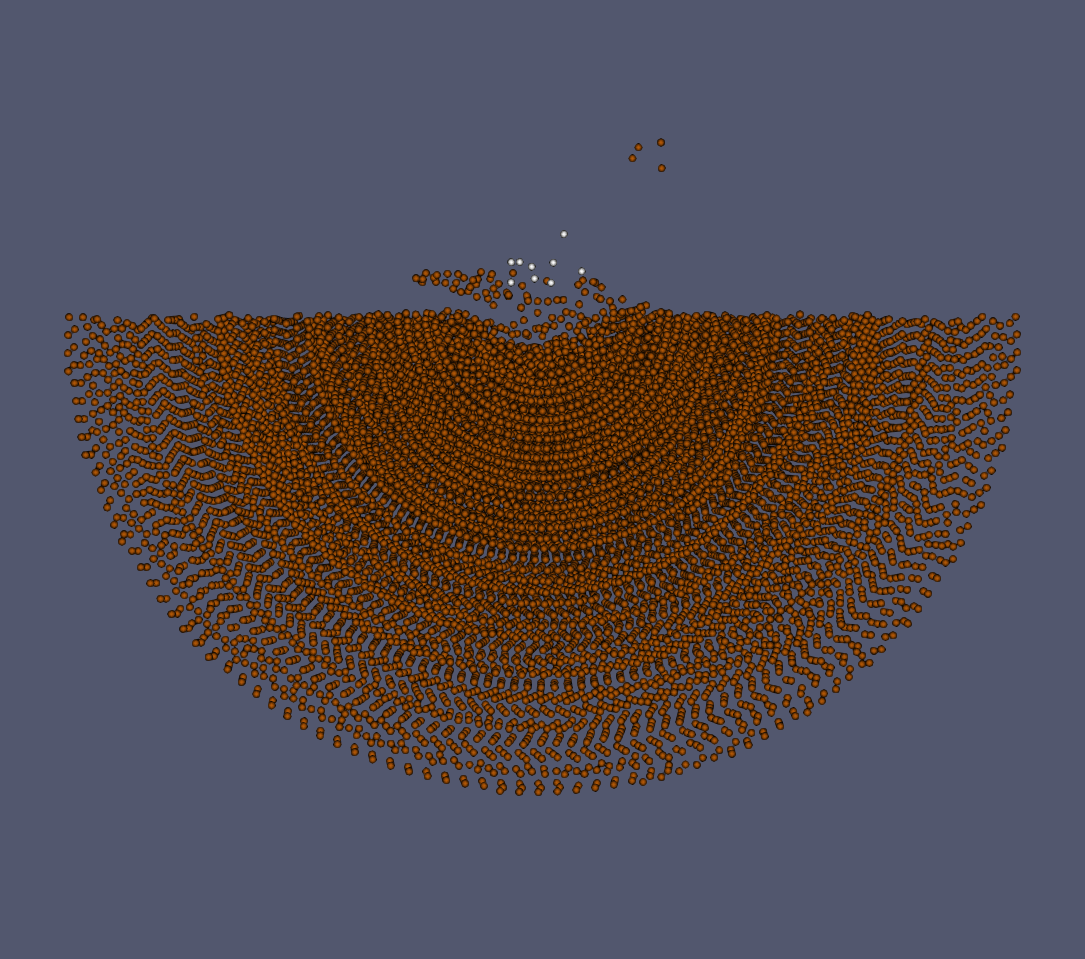
\includegraphics[width=\textwidth]{crater_por0_stre6.png}
   \caption{No porosity (0\%), high strength (Y=1MPa)}
   \label{fig:crater1}
\end{figure}

\begin{figure}[H]
   \centering
   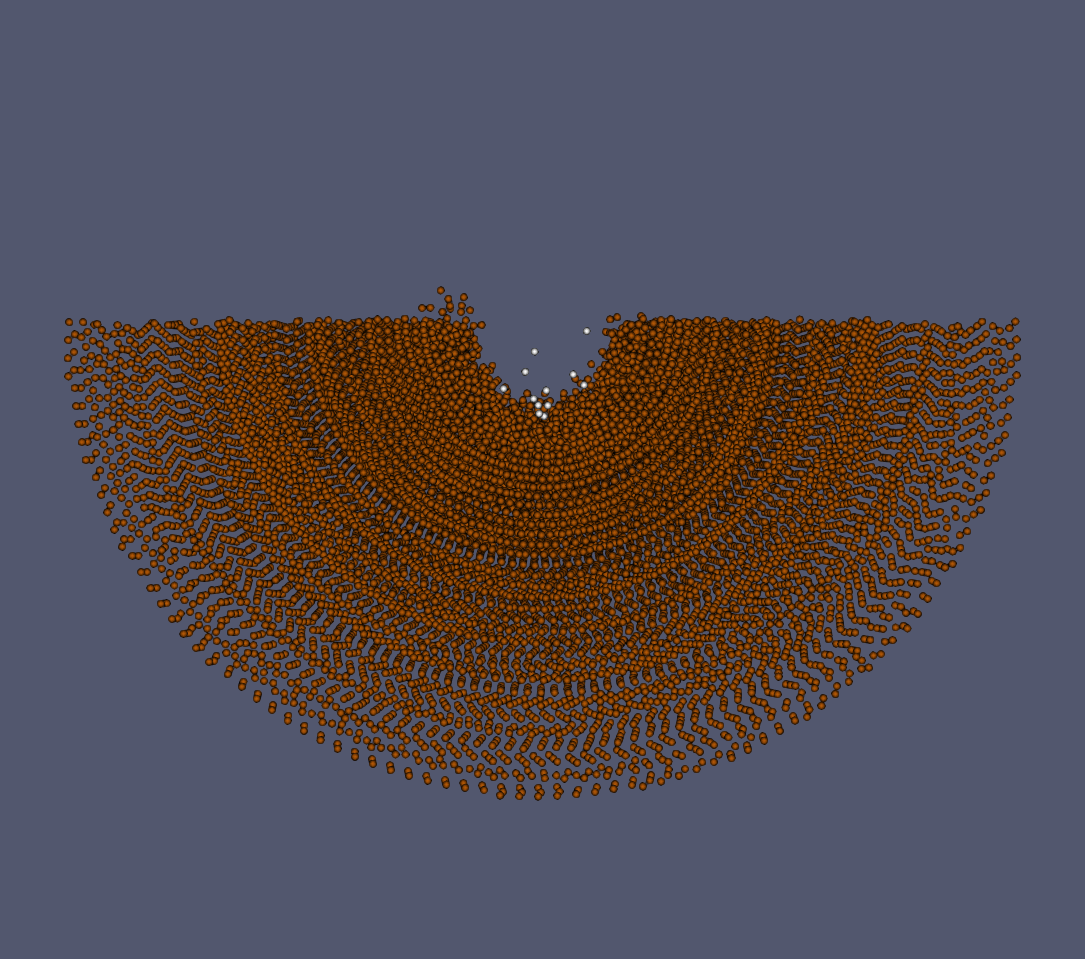
\includegraphics[width=\textwidth]{crater_por50_stre6.png}
   \caption{High porosity (50\%), high strength (Y=1MPa)}
   \label{fig:crater2}
\end{figure}

\begin{figure}[H]
   \centering
   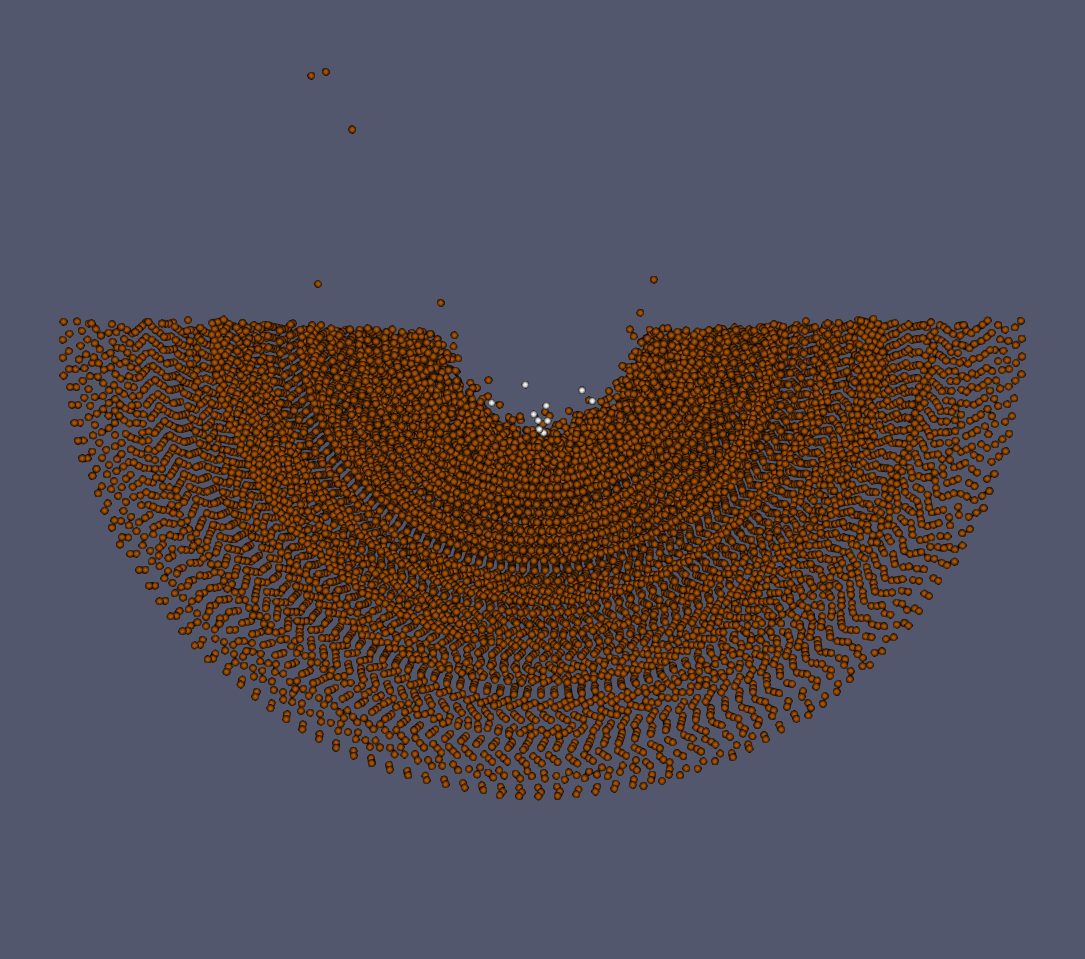
\includegraphics[width=\textwidth]{crater_por50_stre3.png}
   \caption{High porosity (50\%), low strength (Y=1kPa)}
   \label{fig:crater3}
\end{figure}

\begin{figure}[H]
   \centering
   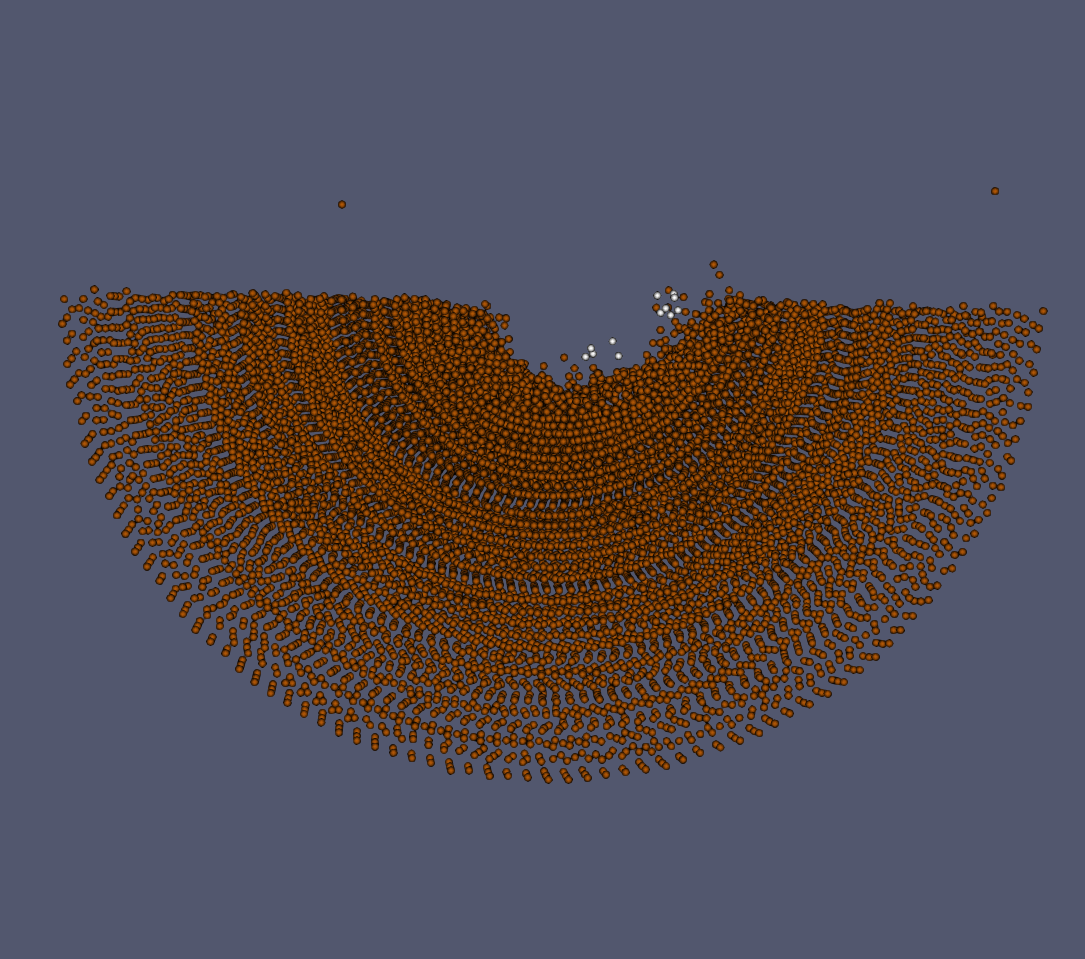
\includegraphics[width=\textwidth]{crater_por50_stre3_ang45.png}
   \caption{High porosity (50\%), low strength (Y=1kPa), 45 degree angle}
   \label{fig:crater4}
\end{figure}


\subsection{Beta factor}
- explanation of beta factor

\begin{figure}[H]
   \centering
   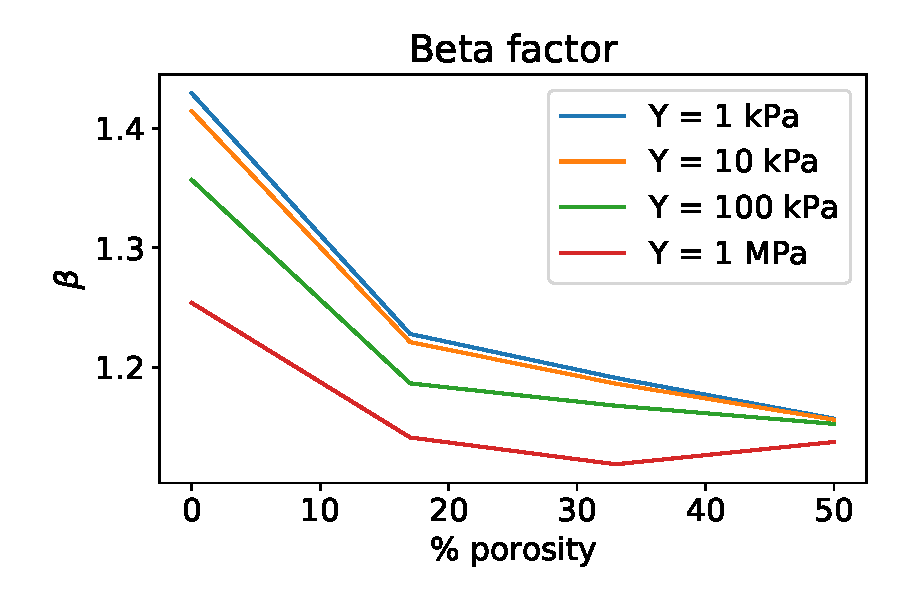
\includegraphics[width=\textwidth]{beta_results.pdf}
   \caption{beta factor}
   \label{fig:beta_factor}
\end{figure}